% Copyright Luke Olson 2009--2014
% This work is licensed under the Creative Commons
% Attribution-NonCommercial-NoDerivatives 4.0 International License. To view a
% copy of this license, visit http://creativecommons.org/licenses/by-nc-nd/4.0/.
%
\documentclass[10pt]{beamer}
%\documentclass[handout,10pt]{beamer}
%
\mode<presentation>
{
  \usetheme[secheader]{Boadilla}
  \usefonttheme[onlymath]{serif}
  \setbeamercovered{invisible}
  \usecolortheme{luke}
  %\setbeamercovered{transparent}
  %
}
\mode<handout>
{
  \usetheme[secheader]{Boadilla}
  \usefonttheme[onlymath]{serif}
  \setbeamercovered{invisible}
  \usecolortheme{luke2}
  %\setbeamercovered{transparent}
}
\usepackage{pgf,pgfarrows,pgfnodes,pgfautomata,pgfheaps,pgfshade}
\usepackage{pxfonts}
\usepackage{eulervm}
\usepackage{listings}
%\usepackage{pgfpages}
%\pgfpagesuselayout{2 on 1}[letterpaper]
%
%
%%%%%%%%%%%%%%%%%%%%%%%%%%%%%%%%%%%%%%%%%%%%%%%%%%%%%%%%%%%%%%%%%%%%%%%%


%
%
%
\newcommand{\vb}{{\bf{b}}}
\newcommand{\ve}{{\bf{e}}}
\newcommand{\vg}{{\bf{g}}}
\newcommand{\vp}{{\bf{p}}}
\newcommand{\vr}{{\bf{r}}}
\newcommand{\vu}{{\bf{u}}}
\newcommand{\vx}{{\bf{x}}}
\newcommand{\vz}{{\bf{z}}}
\newcommand{\vA}{{\bf{A}}}
\newcommand{\vU}{{\bf{U}}}
\newcommand{\mO}{{\mathcal{O}}}
\newcommand{\mF}{{\mathcal{F}}}
\definecolor{mygray}{rgb}{0.95,0.95,0.95}
\lstset{
        language=matlab,
        numbers=left, numberstyle=\tiny, stepnumber=1, numbersep=5pt,
        basicstyle=\color{black}\ttfamily\small,
        commentstyle=\color{green}\ttfamily,
        keywordstyle=\color{blue}\ttfamily,
        stringstyle=\color{red}\ttfamily,
        showstringspaces=false,
        backgroundcolor=\color{mygray},
        breaklines,
}
\newcommand{\norm}[1]{{\ensuremath{{\|#1\|}}}}
\newcommand{\matdim}[2]{\ensuremath{#1\times#2}}
\newcommand{\rank}[1]{\ensuremath{\mathrm{rank}(#1)}}
\newcommand{\epsm}{\ensuremath{\varepsilon_m}}
\newcommand{\cmd}[1]{{\normalfont\ttfamily\bfseries#1}}

\author{L.~Olson}
\institute[UIUC]
{Department of Computer Science\\
University of Illinois at Urbana-Champaign\\
\vspace{0.5cm}
}
%%%%%%%%%%%%%%%%%%%%%%%%%%%%%%%%%%%%%%%%%%%%%%%%%%%%%%%%%%%%%%%%%%%%%%%%
\pgfdeclareimage[height=0.5cm]{university-logo}{./figs/uiuclogo}
\logo{\pgfuseimage{university-logo}}
%%%%%%%%%%%%%%%%%%%%%%%%%%%%%%%%%%%%%%%%%%%%%%%%%%%%%%%%%%%%%%%%%%%%%%%%
\title[CS 357]{Lecture 15}
\subtitle{Interpolation/Splines}
\date{October 15, 2009}

\begin{document}
% -------------------------------------------------
\begin{frame}
  \titlepage
\end{frame}
% -------------------------------------------------
%%%%%%%%%%%%%%%%%%%%%%%%%%%%%%%%%%%%%%%%%%%
\begin{frame}
\frametitle{Recall}
  \begin{block}{}
    Given $n+1$ distinct points $x_0,\dots,x_n$, and values
$y_0,\dots,y_n$, there exists a unique polynomial $p(x)$ of degree at
most $n$ so that
  \begin{equation*}
    p(x_i) = y_i\quad i=0,\dots,n
\end{equation*}
  \end{block}
\end{frame}
%%%%%%%%%%%%%%%%%%%%%%%%%%%%%%%%%%%%%%%%%%%
%%%%%%%%%%%%%%%%%%%%%%%%%%%%%%%%%%%%%%%%%%%
\begin{frame}
\frametitle{Recall: Monomials}
  Obvious attempt: try picking
  \begin{equation*}
    p(x) = a_0 + a_1 x + a_2 x^2 +\dots + a_{n} x^{n}
  \end{equation*}
  So for each $x_i$ we have
  \begin{align*}
    p(x_i) = a_0 + a_1 x_i + a_2 x_i^2 +\dots + a_{n} x_i^{n} & = y_i
  \end{align*}
  OR
  \begin{align*}
    \begin{bmatrix}
      1 & x_0 & x_0^2 & \dots & x_0^{n}\\
      1 & x_1 & x_1^2 & \dots & x_1^{n}\\
        &     &       & \vdots&      \\
      1 & x_n & x_n^2 & \dots & x_n^{n}\\
    \end{bmatrix}
    \begin{bmatrix}
      a_0\\
      a_1\\
      \vdots\\
      a_n\\
    \end{bmatrix}
=
    \begin{bmatrix}
      y_0\\
      y_1\\
      \vdots\\
      y_n\\
    \end{bmatrix}
  \end{align*}
  That is,
\begin{equation*}
  a = M^{-1} y
\end{equation*}

Very bad matrix: terribly ill-conditioned, inverse entries are {\bf{large}}

Very bad evaluation: values are {\bf{huge}}

\end{frame}
%%%%%%%%%%%%%%%%%%%%%%%%%%%%%%%%%%%%%%%%%%%
\begin{frame}
\frametitle{Recall: Shifted Monomials}
  Evaluating
  \begin{equation*}
    p(x) = a_0 + a_1 x + a_2 x^2 +\dots + a_{n} x^{n}
  \end{equation*}
  may have {\bf{huge}} values.  Partial fix:
  \begin{equation*}
    p(x) = a_0 + a_1 (x-\bar{x}) + a_2 (x-\bar{x})^2 +\dots + a_{n} (x-\bar{x})^{n}
  \end{equation*}
  Then $M = vander(x-\bar{x})$ and
  \begin{equation*}
    a = M^{-1} y
  \end{equation*}
  
  Still, a very bad matrix.

\end{frame}
%%%%%%%%%%%%%%%%%%%%%%%%%%%%%%%%%%%%%%%%%%%
\begin{frame}
\frametitle{Recall: Lagrange}
The general Lagrange form is
\begin{equation*}
  \ell_k(x) = \prod_{i=0,i\ne k}^{n} \frac{x-x_i}{x_k - x_i}
\end{equation*}
The resulting interpolating polynomial is
\begin{equation*}
  p(x) = \sum_{k=0}^n \ell_k(x) y_k
\end{equation*}
\end{frame}
%%%%%%%%%%%%%%%%%%%%%%%%%%%%%%%%%%%%%%%%%%%
%%%%%%%%%%%%%%%%%%%%%%%%%%%%%%%%%%%%%%%%%%%
\begin{frame}
\frametitle{Example}
Find the equation of a quadratic passing through the points
(0,-1), (1,-1), and (2,7).

\begin{block}{}
$ x_0 = 0, x_1 = 1, x_2 = 2 \qquad y_0 = -1, y_1 = -1, y_2 = 7 $
\end{block}
\begin{enumerate}
\item Form the Lagrange basis functions, $\ell_i(x)$ with
$\ell_i(x_j)=\delta_{ij}$
\item Combine the Lagrange basis functions
\begin{align*} 
p_2(x)  & =  y_0 \ell_0(x) + y_1 \ell_1(x) + y_2 \ell_2(x) \\ 
        & =  (-1) \frac{(x-1)(x-2)}{2} + (-1)\frac{x(x-2)}{-1} +
(7)\frac{x(x-1)}{2}
\end{align*}
\end{enumerate}

Evaluate is \emph{nice}, but \emph{expensive}: no easy nested form.
\end{frame}
%%%%%%%%%%%%%%%%%%%%%%%%%%%%%%%%%%%%%%%%%%%
%%%%%%%%%%%%%%%%%%%%%%%%%%%%%%%%%%%%%%%%%%%%%%%%%%%%%%%%%%%%%%%%%%%%%%%%
\begin{frame}
\frametitle{Recall: Newton Polynomials}
\begin{itemize}
\item Newton Polynomials are of the form
  \begin{equation*}
    p_n(x) = a_0 + a_1(x-x_0) + a_2(x-x_0)(x-x_1) + a_3(x-x_0)(x-x_1)(x-x_2) + \dots
  \end{equation*}

\item The basis used is thus
\begin{center}
  \begin{tabular}{l l}
  function & order \\
  $1$ & 0\\
  $x-x_0$ & 1\\
  $(x-x_0)(x-x_1)$ & 2\\
  $(x-x_0)(x-x_1)(x-x_2)$ & 3\\
  \end{tabular}
\end{center}

\item More stable evaluation than monomials
\item More computationally efficient (nested iteration) than using Lagrange
\end{itemize}
\end{frame}
%%%%%%%%%%%%%%%%%%%%%%%%%%%%%%%%%%%%%%%%%%%%%%%%%%%%%%%%%%%%%%%%%%%%%%%%%
%%%%%%%%%%%%%%%%%%%%%%%%%%%%%%%%%%%%%%%%%%%%%%%%%%%%%%%%%%%%%%%%%%%%%%%%
\begin{frame}
\frametitle{Fonts == interpolation}
\begin{center}
  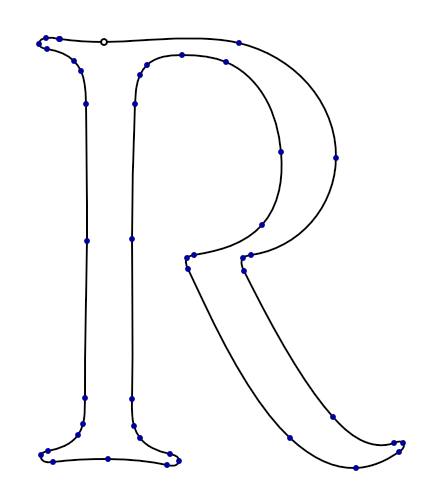
\includegraphics[height=4cm]{./figs/font}
\end{center}
\begin{itemize}
  \item how do we "contain" our interpolation?
  \item splines
  \item Postscript (Adobe): rasterization on-the-fly.  Fonts, etc are defined as
cubic B\'ezier curves (linear interpolation between lower order B\'ezier curves)
  \item TrueType (Apple): similar, quadratic B\'ezier curves, thus cannot
convert from TrueType to PS (Type1) losslessly
\end{itemize}
\end{frame}
%%%%%%%%%%%%%%%%%%%%%%%%%%%%%%%%%%%%%%%%%%%%%%%%%%%%%%%%%%%%%%%%%%%%%%%%
\begin{frame}
\frametitle{How bad is polynomial interpolation?}
  Let's take something very smooth function
\begin{equation*}
  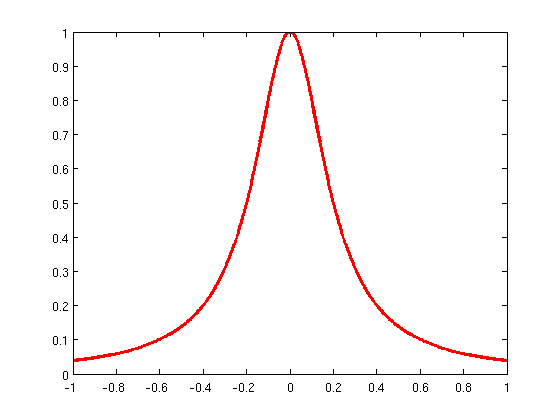
\includegraphics[height=4cm]{./figs/runge}
\end{equation*}

How does interpolation behave?
\end{frame}
\begin{frame}
\frametitle{Some analysis...}
  what can we say about
\begin{equation*}
  e(t) = f(t) - p_n(t)
\end{equation*}
at some point x?  Consider $p=1$: linear interpolation of a function at $x=x_0, x_1$
\begin{itemize}
  \item want: error at $x$, $e(x)$
  \item look at
\begin{equation*}
  g(t) = e(t) - \frac{(t-x_0)(t-x_1)}{(x-x_0)(x-x_1)}e(x)
\end{equation*}
  \item $g(t)$ is 0 at $t=x_0, x_1, x$
  \item so $g'(t)$ is zero at two points
  \item so $g''(t)$ is zero at one point, call it $c$
  \item then
\begin{align*}
  0 & = g''(c) = e''(t) - 2 \frac{e(x)}{(x-x_0)(x-x_1)}\\
    & = f''(t) - 2 \frac{e(x)}{(x-x_0)(x-x_1)}\\
  e(x) &= \frac{(x-x_0)(x-x_1)}{2} f''(c)
\end{align*}
\end{itemize}
\end{frame}
\begin{frame}
\vspace{-0.5cm}
\begin{block}{Theorem: Interpolation Error I}
  If $p_n(x)$ is the (at most) $n$ degree polynomial interpolating $f(x)$ at
$n+1$ distinct points and if $f^{(n+1)}$ is continuous, then 
\begin{equation*}
  e(x) = f(x) - p_n(x) = \frac{1}{(n+1)!} f^{(n+1)}(c) \prod_{i=0}^{n}(x-x_i)
\end{equation*}
\end{block}

\begin{block}{Theorem: Bounding Lemma}
Suppose $x_i$ are equispaced in $[a,b]$ for $i=0,\dots,n$.  Then
\begin{equation*}
  \prod_{i=0}^n |x-x_i| \leq \frac{h^{n+1}}{4} n!
\end{equation*}
\end{block}

\begin{block}{Theorem: Interpolation Error II}
Let $|f^{(n+1)}(x)|\leq M$, then with the above,
\begin{equation*}
  |f(x) - p_n(x)| \leq \frac{M h^{n+1}}{4(n+1)}
\end{equation*}
\end{block}
\end{frame}
\begin{frame}
\frametitle{Fixes}
We have two options:
\begin{enumerate}
  \item move the nodes: Chebychev nodes
  \item piecewise polynomials (splines)
\end{enumerate}
\bigskip
\bigskip

Option \#1: Chebychev nodes in $[-1,1]$
\begin{equation*}
  x_i = cos(\pi \frac{2i+1}{2n+2}), \quad i=0,\dots,n
\end{equation*}
\bigskip

Option \#2: piecewise polynomials...
\end{frame}

\begin{frame}
\frametitle{Chebychev Nodes}
\begin{equation*}
  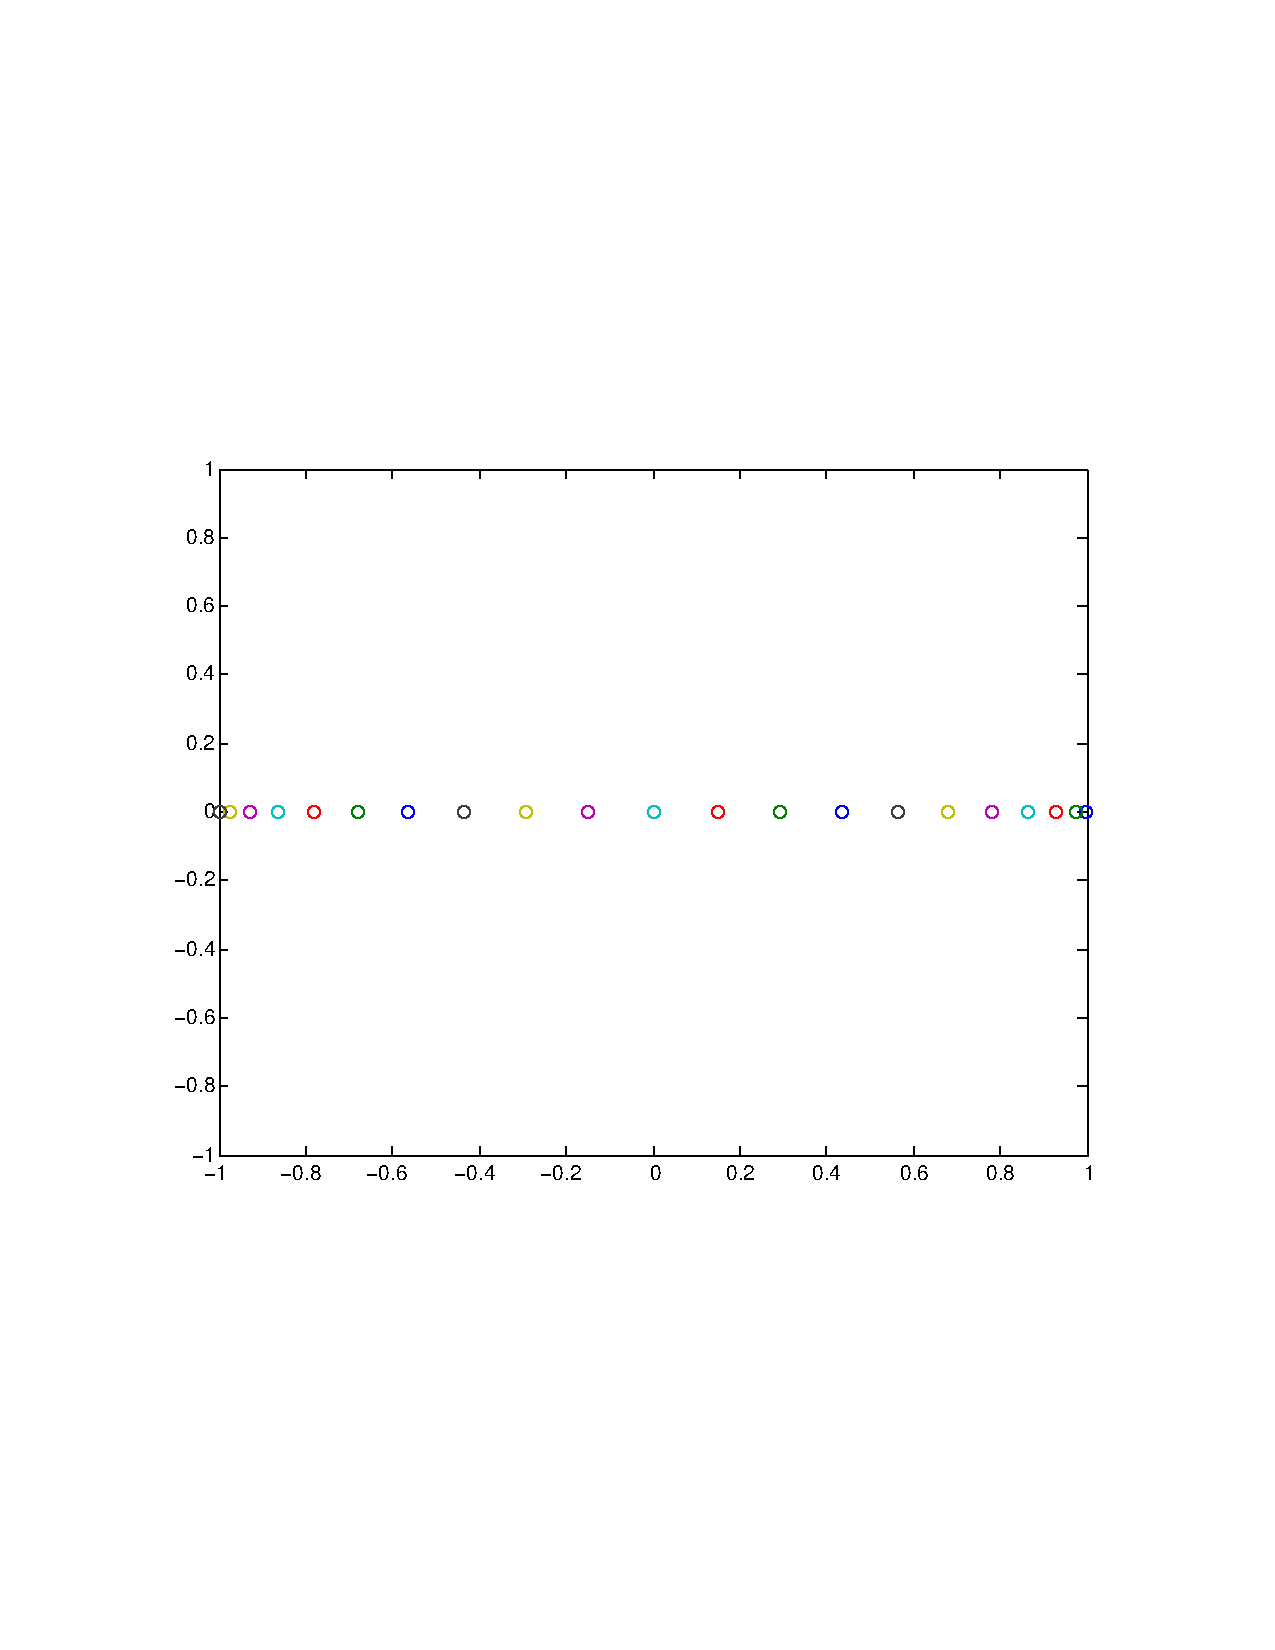
\includegraphics[height=5cm]{./figs/chebychev}
\end{equation*}

\begin{itemize}
\item Can obtain nodes from equidistant points on a circle projected down
\item Nodes are non uniform and non nested
\end{itemize}
\end{frame}
\begin{frame}
\frametitle{Chebychev Nodes}
High degree polynomials using equispaced points suffer from many oscillations
\begin{equation*}
  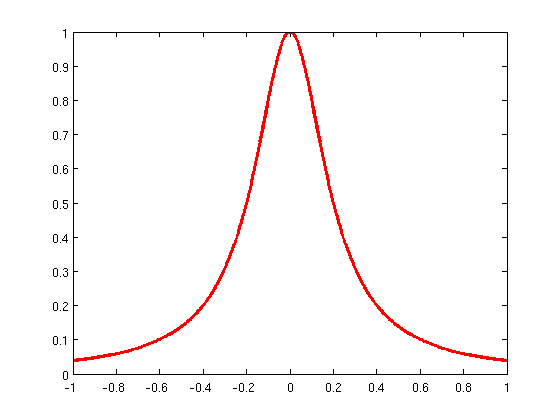
\includegraphics[height=4cm]{./figs/runge}
\end{equation*} 
\begin{itemize}
\item Points are bunched at the ends of the interval 
\item Error is distributed more evenly
\end{itemize}
\end{frame}

%%%%%%%%%%%%%%%%%%%%%%%%%%%%%%%%%%%%%%%%%%%%%%%%%%%%%%%%%%%%%%%%%%%%%%%%
\begin{frame}
\frametitle{Why Splines?}
\begin{columns}
\begin{column}{0.45\textwidth}
\begin{center}
  \pgfimage[width=2.5cm]{./figs/truetype_3}
\end{center}
\begin{center}
  \pgfimage[width=2.5cm]{./figs/utah_teapot}
\end{center}
\begin{center}
  \pgfimage[width=2.5cm]{./figs/spline1}
\end{center}
\end{column}
\begin{column}{0.45\textwidth}
\begin{itemize}
  \item truetype fonts, postscript, metafonts
  \item graphics surfaces
  \item smooth surfaces are needed
  \item how do we interpolate smoothly a set of data?
  \item keywords: Bezier Curves, splines, B-splines, NURBS
  \item basic tool: piecewise interpolation
\end{itemize}
\end{column}
\end{columns}
\end{frame}
%%%%%%%%%%%%%%%%%%%%%%%%%%%%%%%%%%%%%%%%%%%%%%%%%%%%%%%%%%%%%%%%%%%%%%%%
%%%%%%%%%%%%%%%%%%%%%%%%%%%%%%%%%%%%%%%%%%%%%%%%%%%%%%%%%%%%%%%%%%%%%%%%
\begin{frame}
\frametitle{Piecewise Polynomial}
A function $f(x)$ is considered a piecewise polynomial on $[a,b]$ if
there exists a (finite) partition $P$ of $[a,b]$ such that $f(x)$ is a
polynomial on each $[t_i,t_{i+1}]\in P$.

\begin{example}
\begin{equation*}
  f(x) = \begin{cases}
x^3 & x \in [0,1]\\
x & x \in (1,2)\\
3 & x \in [2,3]\\
\end{cases}
\end{equation*}
\end{example}
\begin{center}
  \pgfimage[width=4.5cm]{./figs/pwpoly}
\end{center}
\end{frame}
%%%%%%%%%%%%%%%%%%%%%%%%%%%%%%%%%%%%%%%%%%%%%%%%%%%%%%%%%%%%%%%%%%%%%%%%
%%%%%%%%%%%%%%%%%%%%%%%%%%%%%%%%%%%%%%%%%%%%%%%%%%%%%%%%%%%%%%%%%%%%%%%%
\begin{frame}
\frametitle{What do we want?}
\begin{itemize}
  \item we would like the piecewise polynomial to do two things
  \begin{enumerate}
    \item interpolate (or be close to) some set of data points
    \item look nice (smooth)
  \end{enumerate}
  \item one option is called a \emph{spline}
\end{itemize}
\end{frame}
%%%%%%%%%%%%%%%%%%%%%%%%%%%%%%%%%%%%%%%%%%%%%%%%%%%%%%%%%%%%%%%%%%%%%%%%
%%%%%%%%%%%%%%%%%%%%%%%%%%%%%%%%%%%%%%%%%%%%%%%%%%%%%%%%%%%%%%%%%%%%%%%%
\begin{frame}
\frametitle{splines}
\begin{itemize}
  \item A \emph{spline} is a piecewise polynomial with a certain level of
smoothness.
  \item take Matlab: \texttt{plot(1:7,rand(7,1))}
  \item this is linear and continuous, but not very smooth
  \item the function changes behavior at \emph{knots} $t_0,\dots,t_n$
\end{itemize}
\begin{center}
  \pgfimage[width=4.5cm]{./figs/spline2}
\end{center}
\end{frame}
%%%%%%%%%%%%%%%%%%%%%%%%%%%%%%%%%%%%%%%%%%%%%%%%%%%%%%%%%%%%%%%%%%%%%%%%
%%%%%%%%%%%%%%%%%%%%%%%%%%%%%%%%%%%%%%%%%%%%%%%%%%%%%%%%%%%%%%%%%%%%%%%%
\begin{frame}
\frametitle{degree 1 spline}
\begin{block}{definition}
A function $S(x)$ is a spline of degree 1 if:
\begin{enumerate}
  \item The domain of $S(x)$ is an interval $[a,b]$
  \item $S(x)$ is continuous on $[a,b]$
  \item There is a partition $a=t_0<t_1<\dots<t_n=b$ such that $S(x)$ is
linear on each subinterval $[t_i,t_{i+1}]$.
\end{enumerate}
\end{block}
\begin{columns}
\begin{column}{0.45\textwidth}
\begin{example}
\begin{equation*}
  S(x) = \begin{cases}
  x & x \in [-1,0]\\
  1 & x \in (0,1)\\
  2x-2 & x \in [1,2]\\
\end{cases}
\end{equation*}
\end{example}
\end{column}
\begin{column}{0.45\textwidth}
\begin{center}
  \pgfimage[width=4.5cm]{./figs/spline3}
\end{center}
\end{column}
\end{columns}
\end{frame}
%%%%%%%%%%%%%%%%%%%%%%%%%%%%%%%%%%%%%%%%%%%%%%%%%%%%%%%%%%%%%%%%%%%%%%%%
%%%%%%%%%%%%%%%%%%%%%%%%%%%%%%%%%%%%%%%%%%%%%%%%%%%%%%%%%%%%%%%%%%%%%%%%
\begin{frame}
\frametitle{degree 1 spline}
Given data $t_0,\dots,t_n$ and $y_0,\dots,y_n$, how do we form a spline?
\bigskip
We need two things to hold in the interval $[a,b]=[t_0,t_n]$:
\begin{enumerate}
  \item $S(t_i) = y_i$ for $i=0,\dots,n$
  \item $S_i(x) = a_ix +b_i$ for $i=0,\dots,n$
\end{enumerate}
Write $S_i(x)$ in point-slope form
\begin{align*}
  S_i(x) & = y_i + m_i(x-t_i)\\
         & = y_i + \frac{y_{i+1}-y_i}{t_{i+1}-t_i}(x-t_i)
\end{align*}
Done.
\end{frame}
%%%%%%%%%%%%%%%%%%%%%%%%%%%%%%%%%%%%%%%%%%%%%%%%%%%%%%%%%%%%%%%%%%%%%%%%
%%%%%%%%%%%%%%%%%%%%%%%%%%%%%%%%%%%%%%%%%%%%%%%%%%%%%%%%%%%%%%%%%%%%%%%%
\begin{frame}[fragile]
\frametitle{degree 1 spline}
\begin{lstlisting}[mathescape]
  input $t,y$ vectors of data
  input evaluation location $x$
  find interval $i$ with $x\in[t_i,t_{i+1}]$
  S = y_i + (x-t_i) m_i
\end{lstlisting}
\end{frame}
%%%%%%%%%%%%%%%%%%%%%%%%%%%%%%%%%%%%%%%%%%%%%%%%%%%%%%%%%%%%%%%%%%%%%%%%
%%%%%%%%%%%%%%%%%%%%%%%%%%%%%%%%%%%%%%%%%%%%%%%%%%%%%%%%%%%%%%%%%%%%%%%%
\begin{frame}
\frametitle{degree 1 spline}
Interesting:
\begin{itemize}
  \item input $n+1$ data points $t_0,\dots,t_n$,$y_0,\dots,y_n$
  \item in each interval we have $S_i(x) = a_i x + b_i$
  \item 2 unknowns per interval $[t_i,t_{i+1}]$
  \item or $2n$ total unknowns
  \item the $n+1$ pieces of input contraints $S(t_i)=y_i$ gives 2
constraints per interval
  \item or $2n$ total constraints 
\end{itemize}
\end{frame}
%%%%%%%%%%%%%%%%%%%%%%%%%%%%%%%%%%%%%%%%%%%%%%%%%%%%%%%%%%%%%%%%%%%%%%%%
%%%%%%%%%%%%%%%%%%%%%%%%%%%%%%%%%%%%%%%%%%%%%%%%%%%%%%%%%%%%%%%%%%%%%%%%
\begin{frame}
\frametitle{degree 2 splines}
\begin{block}{definition}
A function $S(x)$ is a spline of degree 2 if:
\begin{enumerate}
  \item The domain of $S(x)$ is an interval $[a,b]$
  \item $S(x)$ is continuous on $[a,b]$
  \item $S'(x)$ is continuous on $[a,b]$
  \item There is a partition $a=t_0<t_1<\dots<t_n=b$ such that $S(x)$ is
quadratic on each subinterval $[t_i,t_{i+1}]$.
\end{enumerate}
\end{block}
\end{frame}
%%%%%%%%%%%%%%%%%%%%%%%%%%%%%%%%%%%%%%%%%%%%%%%%%%%%%%%%%%%%%%%%%%%%%%%%
%%%%%%%%%%%%%%%%%%%%%%%%%%%%%%%%%%%%%%%%%%%%%%%%%%%%%%%%%%%%%%%%%%%%%%%%
\begin{frame}
\frametitle{degree 2 splines}
\begin{equation*}
  S(x) = \begin{cases}
  S_0(x) &  x\in[t_0,t_1]\\
  S_1(x) &  x\in[t_1,t_2]\\
  \vdots & \vdots \\
  S_{n-1}(x) &  x\in[t_{n-1},t_n]\\
\end{cases}
\end{equation*}
for each $i$ we have
\begin{equation*}
  S_i(x) = a_i x^2 + b_i x + c_i
\end{equation*}
What are $a_i$, $b_i$, $c_i$?
\end{frame}
%%%%%%%%%%%%%%%%%%%%%%%%%%%%%%%%%%%%%%%%%%%%%%%%%%%%%%%%%%%%%%%%%%%%%%%%
%%%%%%%%%%%%%%%%%%%%%%%%%%%%%%%%%%%%%%%%%%%%%%%%%%%%%%%%%%%%%%%%%%%%%%%%
\begin{frame}
\frametitle{degree 2 splines}
\begin{itemize}
  \item 3 unknowns in each interval
  \item $3n$ total unknowns
  \item $2n$ constraints for matching up the input data (2 per interval)
  \item $n-1$ interior points require continuity of the derivative:
$S_{i}'(x_{i+1}) = S_{i+1}'(x_{i+1})$
  \item but this is just $n-1$ constraints
  \item total of $3n-1$ constraints
  \item extra consraint: $S'(x_0)=$given, for example.
\end{itemize}
\end{frame}
%%%%%%%%%%%%%%%%%%%%%%%%%%%%%%%%%%%%%%%%%%%%%%%%%%%%%%%%%%%%%%%%%%%%%%%%
%%%%%%%%%%%%%%%%%%%%%%%%%%%%%%%%%%%%%%%%%%%%%%%%%%%%%%%%%%%%%%%%%%%%%%%%
\begin{frame}
\frametitle{degree 3 spline: cubic spline}
\begin{block}{definition}
A function $S(x)$ is a spline of degree 3 if:
\begin{enumerate}
  \item The domain of $S(x)$ is an interval $[a,b]$
  \item $S(x)$ is continuous on $[a,b]$
  \item $S'(x)$ is continuous on $[a,b]$
  \item $S''(x)$ is continuous on $[a,b]$
  \item There is a partition $a=t_0<t_1<\dots<t_n=b$ such that $S(x)$ is
cubic on each subinterval $[t_i,t_{i+1}]$.
\end{enumerate}
\end{block}
\end{frame}
%%%%%%%%%%%%%%%%%%%%%%%%%%%%%%%%%%%%%%%%%%%%%%%%%%%%%%%%%%%%%%%%%%%%%%%%
%%%%%%%%%%%%%%%%%%%%%%%%%%%%%%%%%%%%%%%%%%%%%%%%%%%%%%%%%%%%%%%%%%%%%%%%
\begin{frame}
\frametitle{degree 3 spline: cubic spline}
In each intervale $[t_i,t_{i+1}]$, $S(x)$ looks like
\begin{equation*}
  S_i(x) = a_{0,i} + a_{1,i}x + a_{2,i}x^2 + a_{3,i}x^3
\end{equation*}
\begin{itemize}
  \item<1-> $n$ intervals, $n+1$ knots, 4 unknowns per interval
  \item<1-> $4n$ unknowns
  \item<2-> $2n$ constraints by continuity
  \item<3-> $n-1$ constraints by continuity of $S'(x)$
  \item<4-> $n-1$ constraints by continuity of $S''(x)$
  \item<5-> $4n-2$ total constraints
  \item<6-> This leaves 2 extra degrees of freedom.  The cubic spline is not yet
unique!
\end{itemize}
\end{frame}
%%%%%%%%%%%%%%%%%%%%%%%%%%%%%%%%%%%%%%%%%%%%%%%%%%%%%%%%%%%%%%%%%%%%%%%%
%%%%%%%%%%%%%%%%%%%%%%%%%%%%%%%%%%%%%%%%%%%%%%%%%%%%%%%%%%%%%%%%%%%%%%%%
\begin{frame}
\frametitle{degree 3 spline: cubic spline}
Some options:
  \begin{itemize}
    \item natural cubic spline: $S''(t_0)=S''(t_n)=0$
    \item fixed-slope: $S'(t_0)=a$, $S'(t_n)=b$
    \item not-a-knot: $S'''(x)$ continuous at $t_1$ and $t_{n-1}$
    \item periodic: $S'$ and $S''$ are periodic at the ends
  \end{itemize}
\end{frame}
%%%%%%%%%%%%%%%%%%%%%%%%%%%%%%%%%%%%%%%%%%%%%%%%%%%%%%%%%%%%%%%%%%%%%%%%
%%%%%%%%%%%%%%%%%%%%%%%%%%%%%%%%%%%%%%%%%%%%%%%%%%%%%%%%%%%%%%%%%%%%%%%%
\begin{frame}
\frametitle{natural cubic spline}
How do we find $a_{0,i}, a_{1,i}, a_{2,i}, a_{3,i}$ for each $i$?
\bigskip
Consider knots $t_0,\dots,t_n$.  Follow our example with the following
steps:
\begin{enumerate}
  \item Assume we knew $S''(t_i)$ for each $i$
  \item $S''_i(x)$ is linear, so construct it
  \item Get $S_i(x)$ by integrating $S''_i(x)$ twice
  \item Impose continuity
  \item Differentiate $S_i(x)$ to impose continuity on $S'(x)$
\end{enumerate}

\end{frame}
%%%%%%%%%%%%%%%%%%%%%%%%%%%%%%%%%%%%%%%%%%%%%%%%%%%%%%%%%%%%%%%%%%%%%%%%
%%%%%%%%%%%%%%%%%%%%%%%%%%%%%%%%%%%%%%%%%%%%%%%%%%%%%%%%%%%%%%%%%%%%%%%%
\begin{frame}
\frametitle{natural cubic spline: Step 1}
\framesubtitle{Assume we knew $S''(t_i)$ for each $i$}
We know $S''(x)$ is continuous. So assume
\begin{equation*}
  z_i = S''(t_i) 
\end{equation*}
(we don't actually know $z_i$, not yet at least)
\end{frame}
%%%%%%%%%%%%%%%%%%%%%%%%%%%%%%%%%%%%%%%%%%%%%%%%%%%%%%%%%%%%%%%%%%%%%%%%
%%%%%%%%%%%%%%%%%%%%%%%%%%%%%%%%%%%%%%%%%%%%%%%%%%%%%%%%%%%%%%%%%%%%%%%%
\begin{frame}
\frametitle{natural cubic spline: Step 2}
\framesubtitle{$S''_i(x)$ is linear, so construct it}
Since $S''_i(x)$ is linear, and
\begin{align*}
  S''_i(t_i)&=z_i\\
  S''_i(t_{i+1})&=z_{i+1}
\end{align*}
we can write $S''_i(x)$ as
\begin{align*}
  S''_i(x) & = z_i     \frac{t_{i+1}-x}{t_{i+1}-t_{i}} + 
               z_{i+1} \frac{x-t_{i}}{t_{i+1}-t_{i}}\\
           & = \frac{z_i}{h_i}(t_{i+1}-x) +\frac{z_{i+1}}{h_i}(x-t_i)
\end{align*}

\end{frame}
%%%%%%%%%%%%%%%%%%%%%%%%%%%%%%%%%%%%%%%%%%%%%%%%%%%%%%%%%%%%%%%%%%%%%%%%
%%%%%%%%%%%%%%%%%%%%%%%%%%%%%%%%%%%%%%%%%%%%%%%%%%%%%%%%%%%%%%%%%%%%%%%%
\begin{frame}
\frametitle{natural cubic spline: Step 3}
\framesubtitle{Get $S_i(x)$ by integrating $S''_i(x)$ twice}
Take
\begin{equation*}
  S''_i(x) = \frac{z_i}{h_i}(t_{i+1}-x) +\frac{z_{i+1}}{h_i}(x-t_i)
\end{equation*}
and integrate once:
\begin{equation*}
  S'_i(x) = -\frac{z_i}{2h_i}(t_{i+1}-x)^2
+\frac{z_{i+1}}{2h_i}(x-t_i)^2 + \hat{C}_i
\end{equation*}
twice:
\begin{equation*}
  S_i(x) = \frac{z_i}{6h_i}(t_{i+1}-x)^3
+\frac{z_{i+1}}{6h_i}(x-t_i)^3 + \hat{C}_ix + \hat{D}_i
\end{equation*}
adjust:
\begin{equation*}
  S_i(x) = \frac{z_i}{6h_i}(t_{i+1}-x)^3
+\frac{z_{i+1}}{6h_i}(x-t_i)^3 + C_i(x-t_i) + D_i(t_{i+1}-x)
\end{equation*}
\end{frame}
%%%%%%%%%%%%%%%%%%%%%%%%%%%%%%%%%%%%%%%%%%%%%%%%%%%%%%%%%%%%%%%%%%%%%%%%
%%%%%%%%%%%%%%%%%%%%%%%%%%%%%%%%%%%%%%%%%%%%%%%%%%%%%%%%%%%%%%%%%%%%%%%%
\begin{frame}
\frametitle{natural cubic spline: Step 4}
\framesubtitle{Impose continuity}
For each interval $[t_i,t_{i+1}]$, we require $S_i(t_i)=y_i$ and
$S_i(t_{i+1})=y_{i+1}$:
\begin{align*}
  y_i & = S_i(t_i) = \frac{z_i}{6h_i}(t_{i+1}-t_i)^3
+\frac{z_{i+1}}{6h_i}(t_i-t_i)^3 + C_i(t_i-t_i) + D_i(t_{i+1}-t_i)\\
      & = \frac{z_i}{6}h_i^2 + D_i h_i\\
  D_i & = \frac{y_i}{h_i} - \frac{h_i}{6}z_i\\
\end{align*}
and
\begin{align*}
  y_{i+1} & = S_i(t_{i+1}) = \frac{z_i}{6h_i}(t_{i+1}-t_{i+1})^3
+\frac{z_{i+1}}{6h_i}(t_{i+1}-t_i)^3 + C_i(t_{i+1}-t_i) + D_i(t_{i+1}-t_{i+1})\\
  & = \frac{z_{i+1}}{6}(h_i)^2 + C_ih_i\\
  C_i & = \frac{y_{i+1}}{h_i} - \frac{h_i}{6}z_{i+1}\\
\end{align*}
\end{frame}
%%%%%%%%%%%%%%%%%%%%%%%%%%%%%%%%%%%%%%%%%%%%%%%%%%%%%%%%%%%%%%%%%%%%%%%%
%%%%%%%%%%%%%%%%%%%%%%%%%%%%%%%%%%%%%%%%%%%%%%%%%%%%%%%%%%%%%%%%%%%%%%%%
\begin{frame}
\frametitle{natural cubic spline: Step 4}
\framesubtitle{Impose continuity}
So far we have
\begin{equation*}
  S_i(x) = \frac{z_i}{6h_i}(t_{i+1}-x)^3
+\frac{z_{i+1}}{6h_i}(x-t_i)^3 
+\left(\frac{y_{i+1}}{h_i} - \frac{h_i}{6}z_{i+1}\right)(x-t_i)
+\left(\frac{y_i}{h_i} - \frac{h_i}{6}z_i\right) (t_{i+1}-x)
\end{equation*}
\end{frame}
%%%%%%%%%%%%%%%%%%%%%%%%%%%%%%%%%%%%%%%%%%%%%%%%%%%%%%%%%%%%%%%%%%%%%%%%
%%%%%%%%%%%%%%%%%%%%%%%%%%%%%%%%%%%%%%%%%%%%%%%%%%%%%%%%%%%%%%%%%%%%%%%%
\begin{frame}
\frametitle{natural cubic spline: Step 5}
\framesubtitle{Differentiate $S_i(x)$ to impose continuity on $S'(x)$}
\begin{equation*}
  S'_i(x) = -\frac{z_i}{2h_i}(t_{i+1}-x)^2
+\frac{z_{i+1}}{2h_i}(x-t_i)^2 
+\frac{y_{i+1}}{h_i} - \frac{h_i}{6}z_{i+1}
-\frac{y_i}{h_i} + \frac{h_i}{6}z_i
\end{equation*}
We need $S'_i(t_i) = S'_{i-1}(t_i)$:
\begin{equation*}
  S'_i(t_i) = -\frac{h_i}{6}z_{i+1}
              -\frac{h_i}{3}z_i
              +\underbrace{\frac{1}{h_i}(y_{i+1}-y_i)}_{b_i}
\end{equation*}
\begin{equation*}
  S'_{i-1}(t_i) = \frac{h_{i-1}}{6}z_{i-1}
              +\frac{h_{i-1}}{3}z_i
              +\underbrace{\frac{1}{h_{i-1}}(y_{i}-y_{i-1})}_{b_{i-1}}
\end{equation*}
Thus $z_i$ is defined by
\begin{equation*}
  h_{i-1}z_{i-1} + 2(h_i+h_{i-1})z_i + h_{i}z_{i+1} = 6(b_i-b_{i-1})
\end{equation*}
\end{frame}
%%%%%%%%%%%%%%%%%%%%%%%%%%%%%%%%%%%%%%%%%%%%%%%%%%%%%%%%%%%%%%%%%%%%%%%%
%%%%%%%%%%%%%%%%%%%%%%%%%%%%%%%%%%%%%%%%%%%%%%%%%%%%%%%%%%%%%%%%%%%%%%%%
\begin{frame}
\frametitle{natural cubic spline: Step 6}
\framesubtitle{solve}
$z_i$ is defined by
\begin{equation*}
  h_{i-1}z_{i-1} + 2(h_i+h_{i-1})z_i + h_{i}z_{i+1} = 6(b_i-b_{i-1})
\end{equation*}
\begin{itemize}
  \item This is $n-1$ equations, $n-1$ unknowns ($z_0=z_n=0$ already)
  \item an $(n-1)\times (n-1)$ tridiagonal system
\end{itemize}
\[
\begin{bmatrix}
 1 &  & & & & & & \\ 
 h_0 & u_1  & h_1 & & & & & \\ 
 & h_1            &  u_2 & h_2 & & & & \\ 
 &                & h_2             & u_3 & h_3  & & & \\ 
 &                &                 & \ddots  & \ddots & \ddots & & \\  
 &  &   &   & h_{n-3} & u_{n-2} & h_{n-2}  & \\ 
 &  &   &   &         & h_{n-2} &  u_{n-1}& h_{n-1}\\
 &  &   &   &         &         &        & 1\\
\end{bmatrix}
\begin{bmatrix}
z_0\\z_1\\  z_2\\  z_3\\  \vdots\\  z_{n-2}\\  z_{n-1}\\z_n\\
\end{bmatrix}
 = 
\begin{bmatrix}
0\\v_1\\  v_2\\  v_3\\  \vdots\\  v_{n-2}\\  v_{n-1}\\0\\
\end{bmatrix}
\] 
 
\begin{eqnarray*}
u_i & = & 2 (h_i + h_{i-1} ) \\
v_i & = & 6(b_i - b_{i-1})
\end{eqnarray*} 
\end{frame}
%%%%%%%%%%%%%%%%%%%%%%%%%%%%%%%%%%%%%%%%%%%%%%%%%%%%%%%%%%%%%%%%%%%%%%%%
%%%%%%%%%%%%%%%%%%%%%%%%%%%%%%%%%%%%%%%%%%%%%%%%%%%%%%%%%%%%%%%%%%%%%%%%
\begin{frame}
\frametitle{example}
Find the natural cubic spline for 
\begin{tabular}{c | c c c }
$x$ & -1 & 0 & 1\\\hline
$y$ & 1 & 2 & -1\\
\end{tabular}
\begin{enumerate}
  \item Determine $h_i$, $b_i$, $u_i$, $v_i$
    \begin{equation*}
  h=
  \begin{bmatrix}
    1\\1\\
  \end{bmatrix}\quad
  b=
  \begin{bmatrix}
    1\\-3\\
  \end{bmatrix}\quad
  u=
  \begin{bmatrix}
    4\\
  \end{bmatrix}\quad
  v=
  \begin{bmatrix}
    -24
  \end{bmatrix}
    \end{equation*}
  \item Solve
  \begin{equation*}
  \begin{bmatrix}
    1 & &\\
    1&4&1\\
    & & 1\\ 
  \end{bmatrix}
  \begin{bmatrix}
    z_0\\
    z_1\\
    z_2\\
  \end{bmatrix}
=
  \begin{bmatrix}
    0\\
    -24\\
    0\\
  \end{bmatrix}
  \end{equation*}
  \item Result:
  \begin{equation*}
  \begin{bmatrix}
    z_0\\
    z_1\\
    z_2\\
  \end{bmatrix}
=
  \begin{bmatrix}
    0\\
    -6\\
    0\\
  \end{bmatrix}
  \end{equation*}
\end{enumerate}
\end{frame}
%%%%%%%%%%%%%%%%%%%%%%%%%%%%%%%%%%%%%%%%%%%%%%%%%%%%%%%%%%%%%%%%%%%%%%%%
%%%%%%%%%%%%%%%%%%%%%%%%%%%%%%%%%%%%%%%%%%%%%%%%%%%%%%%%%%%%%%%%%%%%%%%%
\begin{frame}
\frametitle{example}
Find the natural cubic spline for 
\begin{tabular}{c | c c c }
$x$ & -1 & 0 & 1\\\hline
$y$ & 1 & 2 & -1\\
\end{tabular}
\begin{enumerate}
  \item Plug $z_i$ into
\begin{eqnarray*}
  S_i(x) &=& \frac{z_i}{6h_i}(t_{i+1}-x)^3
+\frac{z_{i+1}}{6h_i}(x-t_i)^3 
+\left(\frac{y_{i+1}}{h_i} - \frac{h_i}{6}z_{i+1}\right)(x-t_i)\\
&&+\left(\frac{y_i}{h_i} - \frac{h_i}{6}z_i\right) (t_{i+1}-x)
\end{eqnarray*}
\bigskip

\begin{equation*}
  S(x) = \begin{cases}
    -(x+1)^3 + 3(x+1)-x& -1\leq x < 0\\ 
    -(1-x)^3 -x +3(1-x)& 0\leq x < 1\\ 
\end{cases}
\end{equation*}
\end{enumerate}
\end{frame}
%%%%%%%%%%%%%%%%%%%%%%%%%%%%%%%%%%%%%%%%%%%%%%%%%%%%%%%%%%%%%%%%%%%%%%%%
%%%%%%%%%%%%%%%%%%%%%%%%%%%%%%%%%%%%%%%%%%%%%%%%%%%%%%%%%%%%%%%%%%%%%%%%
\begin{frame}
\frametitle{Algorithm: page 391 NMC6 (page 403, NMC5)}
\begin{enumerate}
  \item Compute for $i=0,\dots,n-1$
  \begin{equation*}
  h_i=t_{i+1}-t_i\qquad b_i=\frac{1}{h_i}(y_{i+1}-y_{i})
  \end{equation*}
  \item Set $u$, $v$:
  \item tridiagonal solve to get $z$
  \item substitute into the nested form for $S(x)$ equation 12, page 392 NMC6 (NMC5: equation 10 page 404)
\end{enumerate}
\end{frame}
%%%%%%%%%%%%%%%%%%%%%%%%%%%%%%%%%%%%%%%%%%%%%%%%%%%%%%%%%%%%%%%%%%%%%%%%
%%%%%%%%%%%%%%%%%%%%%%%%%%%%%%%%%%%%%%%%%%%%%%%%%%%%%%%%%%%%%%%%%%%%%%%%
\begin{frame}
\frametitle{Next time...}
  \begin{itemize}
  \item more on the cubic algorithm
  \item the B-splines/Bezier Curves
\end{itemize}
\end{frame}
%%%%%%%%%%%%%%%%%%%%%%%%%%%%%%%%%%%%%%%%%%%%%%%%%%%%%%%%%%%%%%%%%%%%%%%%
\end{document}

\end{document}
